\documentclass[11pt]{article}
\usepackage{graphicx}
\usepackage[pdf]{pstricks}
%\usepackage{mathtools}
\usepackage{amssymb,amsmath}
\usepackage{textcomp}
\DeclareMathOperator*{\argmin}{arg\,min}

%\usepackage{subcaption}
%\usepackage{float}
\usepackage{setspace}
\usepackage{fullpage}
\usepackage[font=scriptsize]{caption}
%\usepackage{fullpage}
%\setcounter{secnumdepth}{1}
\begin{document}

\title{Fused regression for multi-source network inference}
\author{Kari Y. Lam, Zachary M. Westrick, Christian L. M\"{u}ller, Lionel Christiaen, Richard Bonneau}
\maketitle

\begin{abstract}
Understanding gene regulatory networks is critical to learning how cells regulate their behavior and respond to external stimuli. To this end, methods for global network inference have been developed and applied to a variety of species. However, most approaches consider the problem of network inference independently in each species, despite evidence that gene regulation is conserved even in distantly related species. We introduce a method for multi-source network inference that allows simultaneous estimation of gene regulatory networks in multiple species or biological processes through the incorporation of priors based on known gene relationships such as orthology. This approach improves network inference performance even when the orthology mapping in incomplete. We further refine this method with an algorithm that attempts to learn the true conserved subnetwork from a larger set of potentially conserved interactions. We demonstrate the utility of our method not only in cross species network inference, but also in merging data collected on different experimental platform and in incorporating binding similarity predictions.
\end{abstract}

\section{Introduction}
As the volume and variety of genome scale data have exploded, the goal of accurately modeling gene regulatory networks has become more attainable \cite{bonneau_predictive_2007, ciofani_validated_2012, carro_transcriptional_2010}. Large-scale data collection efforts have contributed to the development of high quality networks, but there remain many biological processes and organisms for which there does not exist adequate data. Furthermore, as new technologies are developed and some old ones are replaced, such as RNAseq and microarray, it becomes important to be able to combine data from multiple platforms, lest we lose valuable information from existing studies. The problem of inferring related -- but not necessarily identical -- structure from related -- but not identical -- data is ubiquitous in biology. Multi-source network inference has applications for learning multiple networks in multiple related species, for learning networks associated with distinct processes within the same species, and for learning networks based on heterogenous data sources.

Moreover, as it becomes increasingly possible to learn genome-wide regulatory networks, we can begin to compare and to test whether there is conservation of networks across species and biological processes. Our use of model organisms to study biological processes and diseases relevant to humans relies on the assumption of conservation; yet this has not been tested at the genome scale. 

We present two methods for network inference based on linear estimates of gene expression dynamics, extending existing linear dynamical-systems methods for network inference \cite{bonneau_predictive_2007, arrieta-ortiz_experimentally_2015}. The core of both methods is the observation that biological information about the relatedness of two networks can be used to constrain which network coefficients should be similar to one another in a multi-source network inference problem (ie orthologous TFs should regulate orthologous genes), and that these constraints can be efficiently represented as penalties in a least-squares regression problem. Our first method -- fused ridge -- uses an L2 penalty on the differences between a priori similar interactions, and is useful where the relationships between networks (similarity of genes between data sets) is reliable. In the case where both networks contain an identical set of genes and TFs, this approach can be thought of as parametrically interpolating between treating the data sources separately and combining them together. However, our method allows useful pooling of data even when the overlap between genes is incomplete. Our second method -- adaptive fusion -- uses a non-concave saturating fusion penalty to simultaneously learn the constrained networks and to learn which constraints should be relaxed (ie which parts of the network are genuinely different). With this approach, we seek to test the hypothesis of conservation of interactions across networks.

In the case of multiple species, there has been a great deal of work showing that functional conservation exists in gene regulatory networks even across large evolutionary distance \cite{satou2006gene, hinman2009evolution,tanay2005conservation,erwin2009evolution}. In our fused L2 approach, we make the assumption that if a pair of TFs is orthologous to one another, then their regulatory effects on a pair of orthologous genes should be similar. These orthology relationships form the basis of a set of constraints which favor -- but do not require -- networks in which orthologous transctiption factors regulate orthologous genes. As a result, data in one species can improve network inference performance in another species  (and vice versa). This general framework for multi-species network inference can be extended to an arbitrary number of distinct organisms, each contributing data with only partially overlapping sets of genes. This is an advantage over existing approaches to multi-species network inference, which infer only a sub-network for which orthologs exist in every species \cite{joshi_multi-species_2015}. This approach of introducting constraints on the similarity between specific regulatory interactions can be extended beyond the case of multi-species network-inference from orthology; any biological prior on similarity can be used in place of orthology. For example, we can introduce constraints that favor genes in the same operon or having similar binding sites, having similar regulators.

Existing multi species approaches often use orthology as a proxy for functional conservation \cite{penfold_inferring_2015, joshi_multi-species_2015, kashima_simultaneous_2009, zhang2010nearly}, or attempt to learn functional similarity via expression data \cite{gholami_cross-species_2010}. Orthology -- the measure of gene similarity we use -- can be approximated using readily identifiable sequence similarity. Sequence similarity is often a useful predictor of functional similarity \cite{wilson_assessing_2000}. In multi-species network inference, our fused L2 approach minimizes a cost function that strives to simultaneously fit expression data in each species and produce networks that are consistent with evolutionary constraints created using orthology. However, we recognize that some genes may have taken on different functions and therefore may have new regulatory interactions. Gene duplications and neofunctionalization in multi-species network inference \cite{eisen_phylogenomics:_1998}, and changes in chromatin configuration in multi-cell line network inference \cite{li_role_2007}, are cases where enforcing fusion of constraints does not produce networks which reflect true differences in regulation between networks. These cases can be difficult to learn by simply comparing independently inferred networks; because network inference is typically underconstrainted \cite{marbach_revealing_2010-1}, there could be other plausible networks in which the coefficients being compared are similar. Our adaptive fusion method allows us to learn differences in networks predicted to be similar based on orthology or gene matching: because the constraints we impose favor weight configurations in which fused interaction weights are similar to one another, a solution in which a priori similar regulatory interactions are found to be different is strong evidence that they really are different. When differences in regulatory interactions arise where they are predicted to be similar, the network inference procedure would be improved by relaxing or ignoring these evolutionary constraints. However, we don't know a priori which constraints to enforce and which to relax. 

We approach this problem by introducing a saturating penalty function based on work in statistics to develop unbiased regularization penalties for regression \cite{zhang2010nearly, fan2001variable}. The main difference between the L2 fusion approach and this adaptive fusion approach occurs when the difference between presumed analogous interactions is large despite the fusion penalty: we assume that large differences represent evidence that gene functions have diverged and represent this, in adaptive fusion, with a relaxation of the fusion penalty. The resulting cost function is non-convex and difficult to optimize; however, we can approximate its solution and obtain deeper insights into functional similarity than is available through orthology or the comparison of separately learned networks. 

We test the ability of fused L2 and adaptive fusion to improve network recovery on both synthetic data and Bacillus subtilis and Bacillus anthracis, showing the applicability of our method in combining different datasets, and leveraging similarity across organisms as well as within a network in order to improve network inference. We explore the circumstances under which each approach is optimal, and evaluate the robustness of adaptive fusion to incorrect orthology, simulating the biologically relevant case of neofunctionalization. 

\section{Methods}
\subsection{Gene regulatory network}
We model each gene's expression as a linear combination of transcription factors (TFs), and we seek to identify the TFs which regulate each gene, and the strength of the TF-gene interactions. In the Inferelator algorithm, linear differential equations are used to model changes in gene expression \cite{bonneau_inferelator:_2006-1} Our primary data for learning gene regulatory networks is expression data, time-series and steady state experiments. We use time-series data to approximate the rate of change of expression, and we treat steady-state experiments as conditions that have reached equilibrium. The rate at which $x_{i}$, the observed mRNA expression of gene $i$, changes, is governed by degradation of existing transcripts with rate $\alpha$ plus a linear combination of transcription factor (TF) expressions. 
\begin{equation}
\frac{\mathrm d}{\mathrm d t} x_i = -\alpha_{i}x_{i} + \sum \beta_{i,j}x_{j}
\end{equation}
where $\beta_{i,j}$ represents the weight of TF $j$ on gene $i$, and $\alpha$ is the decay rate of gene $i$. We fix the decay rate $\alpha$ for all genes, and set it assuming a time-constant of 10 minutes \cite{hambraeus_genome-wide_2003, selinger_global_2003}, as in \cite{greenfield_robust_2013}. Let $x_i(t)$ be the expression of gene $i$ at time $t$. Given time-series data on the expression of gene $i$ at timepoints $t_k$ and $t_{k+1}$, we can approximate the rate of change of $x_i$ as $x_i'(t_k)=\frac{x_i(t_{k+1})-x_i(t_k)}{t_{k+1}-t_k}$. We treat steady-state data as having a derivative of zero. This gives us, for each gene $i$ and time $t_{k}$ an equation

\begin{equation}
\frac{x_i(t_{k+1})-x_i(t_k)}{t_{k+1}-t_k} + \alpha_{i}x_{i}(t_k)= \sum \beta_{i,j}x_{j}(t_k)
\end{equation}
\noindent We can summarize these equations in matrix form as
\begin{equation}
Y = X \beta 
\end{equation}

We are interested in learning $\beta$, the matrix representation of the gene regulatory network, where the weight in a given position represents the regulatory weight of a TF on a gene. Positive weights represent activation, negative weights represent repression, and 0 weights represent the absence of an interaction. 

\noindent We approach the learning of the $\beta$ matrix using regression. Because there are typically far fewer conditions than possible regressors (TFs), we introduce a ridge regularization constraint with weight $\lambda_R$ and solve
\begin{equation}
\argmin_\beta\vert \vert X\beta - Y_2 \vert \vert ^2 + \lambda_R \vert \vert \beta \vert \vert ^2
\end{equation}
This is similar to the formulation used in the Inferelator algorithm, which we extend to the case of simultaneously inferring the GRNs of multiple species. 

\subsection{Fused gene regulatory networks}
We hypothesize that related species should be governed by similar but not necessarily identical gene regulatory networks. We approach the problem of cross-species GRN inference by introducing constraints into the above regression formulation to penalize differences between interaction weights that are expected to be similar based on, say, gene orthology. We can then solve the penalized regression problems simultaneously, in order to obtain a GRN for each species. Consider the case of organisms $A$ and $B$, governed by GRNs $\beta^A$ and $\beta^B$ (the following approach applies equally well to more than two species but for simplicity we continue with the case of two species). If TF $g^A$ in organism $A$ and TF $h^B$ in organism $B$ are orthologs, and gene $k^A$ and $l^B$ are orthologs, then we expect that the $g^A \rightarrow k^A$ interaction weight should be similar to the $h^B \rightarrow l^B$ interaction weight, and we introduce a fusion constraint between these analogous interactions. In terms of the above regression formulation, we expect that $\beta^A_{g,k} \approx \beta^B_{h,l}$, and include a penalty term $p_{\lambda_S}(\beta^A_{g,k} - \beta^B_{h,l})$ to the quantity being minimized in order to ensure similarity. The parameter $\lambda_S$ controls how highly to penalize differences between fused coefficients and controls the tradeoff between fitting the expression data and producing a set of networks that conform to evolutionary constraints. This gives us the final equation to be minimized 
\begin{equation}
%\argmin_{(\beta^A, \beta^B)} \displaystyle\sum_{S \in (A, B)} \vert \vert X^S\beta^S - Y^S \vert \vert ^2 + \lambda_R \vert \vert \beta^S \vert \vert ^2 + \displaystyle \sum_{\beta^{S_1}_{g,k} \approx \beta^{S_2}_{h,l}} p_{\lambda_S}(\beta^{S_1}_{g,k} - \beta^{S_2}_{h,l})
\argmin_{(\beta^A, \beta^B)} \displaystyle\sum_{S \in (A, B)} \vert \vert X^S\beta^S - Y^S \vert \vert ^2 + \lambda_R \vert \vert \beta^S \vert \vert ^2 + \displaystyle \sum_{\substack{(g,h) \in orth,\\
 (h,l) \in orth}}x p_{\lambda_S}(\beta^{S_1}_{g,k} - \beta^{S_2}_{h,l})
\end{equation}

where the second sum is over pairs of interactions with fusion constraints. 


\subsection{Fused L2 penalty for multi-source network inference}
When the penalty $p_{\lambda_S}$ is the L2 norm, as in our fused L2 approach:
\begin{equation}
\argmin_{(\beta^A, \beta^B)} \displaystyle\sum_{S \in (A, B)} \vert \vert X^S\beta^S - Y^S \vert \vert ^2 + \lambda_R \vert \vert \beta^S \vert \vert ^2 + \displaystyle \lambda_S \sum_{\substack{(g,h) \in orth,\\
 (h,l) \in orth}} \vert \vert (\beta^{S_1}_{g,k} - \beta^{S_2}_{h,l}) \vert \vert ^2
\end{equation}

the entire problem can be solved through linear regression with a suitable design matrix. The regulators of a pair of genes can be solved independently as long as the pair is not linked by fusion constraints, or a chain of fusion constraints; thus the problem of cross-species GRN inference decomposes into a large number of manageable regression problems as long as the orthology mappings are sparse.

In order to better understand this, consider the case where there is a one-to-one orthology between the species being considered (ie different cell-lines of the same organism). The choice of $\lambda_S$ allows one to interpolate between fitting each network independently ($\lambda_S=0$) and pooling data together as if it came from one source ($\lambda_S=\inf$). Part of the appeal of the approach, however, is that it allows pooling of data even when there is incomplete orthology. By introducing constraints on the similarity of individual interactions, rather than on the networks as a whole \cite{liu2011temporal}, we can pool some information across species even when an arbitrarily small fraction of genes have orthologs. This is particularly useful when dealing with a large number of species; pairwise orthologies may be nearly complete even when the number of genes present in every organism is small. 

\subsection{Solving fused L2 problems using augmented matrices}
We use the fact that ridge regression can be solved by ordinary least squares regression on an augmented dataset, by appending a scaled identity matrix to the design matrix, and zeros to the response matrix. The problem of solving a multi-valued regression problem can also be converted into the problem of solving a single valued regression problem by vectorization. 

Specifically, if $Y \in R^{N \times M}$ then we form $A =$ diagonally concatenate $X$, $M$ times (with the remaining entries 0),
$y =$ vertically concatenate the columns of $Y$. We solve 

$$\underset{W}{min} ||AW - y||_2^{~2}$$

%We can then define $W_{i,j} = \beta_{(j-1) \times N + i, (j-1) \times M + j}$ which is the desired form.
This is equivalent to the original problem due to the block structure of matrix multiplication. In an ordinary ridge regression problem, this is unnecessary, as the columns of the weight matrix can be solved independently. However, in fused regression, information is shared between columns, and therefore they must be solved for simultaneously. If two entries are in the same fusion constraint, or if there exists a constraint chain containing entries from two columns, those columns must be solved together. Two entries may be fused if say, two TFs are orthologous, and two genes are orthologous--then, the interaction between the first TF, gene pair should be similar to the second TF, gene pair. A constraint chain can exist if there are complex orthology mappings, say, if there are multiple similar sequence signals, and three or more entries are fused. 

%Given $X_1... X_S$ matrices, $X_i \in R^{N_i \times K_i}$ we define $N = \sum_{i=0}^S N_i$, $K = \sum_{i=0}^SK_i$ and $X \in R^{N \times K}$ by diagonally concatenating $X_1...X_S$.
%In this new matrix, the first $K_1$ features correspond to features of $X_1$, the next $K_2$ features the features of $X_2$ etc.
%Similarly, the first $N_1$ samples correspond to samples of $X_1$, the next $N_2$ to $X_2$ etc.
%Solving the regression problem associated with each source is equivalent to solving the problem $\underset{W}{argmin}||XW-Y||$ where $Y$ is defined in the same way as $X$.
%The weight matrix $W$ has a block diagonal structure:

%\begin{figure}[h!]
%    \centering
%    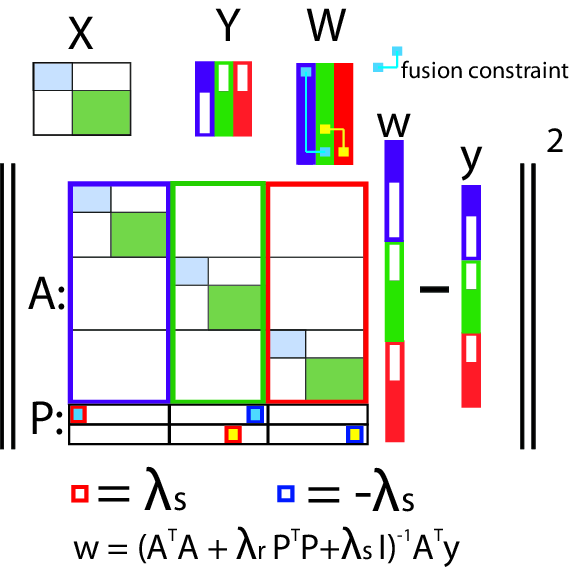
\includegraphics[scale=.5,trim=0mm 0mm 0mm 0mm,clip]{direct_solve.png}
%\end{figure}

The fused multi-source regression problem can solved by constructing a multi-source design matrix $X$ and data matrix $Y$, and then vectorizing.
Suppose we have a constraint with the form

%The regression problems associated with two columns $A,A'$ of $Y$, where $A$ came from $Y_1$ and $A'$ came from $Y_2$, are independent, unless there is a constraint chain of length $L$ with the form

%$$(G, j_0, g, J_1, j_1, m_1) \rightarrow (J_1, j_1, m_1, J_2, j_2, m_2) \rightarrow (J_2,j_2,m_2,J_3,j_3,_m3)...(J_P, j_P, m_P, H, j_{P+1}, h)$$
%$$(Y_1, j_1, g, Y_2, j_2, h) \rightarrow (Y_2, j_2, h, Y_3, j_3, k)$$
$((\beta_1, A, B), (\beta_1, A, C), (\beta_2, A', B'))$

Here, we have two datasets, which we refer to as 1 and 2. We have information about the similarity of TF A in network 1 to TF A' in network 2, and about the similarity of genes B and C in network 1 to gene B' in network 2. We expect, therefore, that if an interaction exists between A and B or A and C in the first network, that these interactions be similar to the interaction between A' and B' in the second network, and we penalize solutions which do not have this feature. 

To find all such linked problems, we use depth-first search to identify linked columns of the TF expression matrix $Y$, then solve the fused regression problem directly by vectorizing corresponding columns. To incorporate the fusion penalty, we append to the resulting block diagonal design matrix one row per connected constraint, which contains $\lambda_S$ in the column associated with the TF, gene pair (A, B) from dataset 1, and $-\lambda_S$ to the column associated with TF, gene pair (A', B') from dataset 2, as well as another one for (A, C), (A', B'). The vector $Y$ is augmented by appending an appropriate number of zeros. This results in the addition of the penalties, $\lambda_S||b_{A,B} - b_{A',B'}||^{2}$ and $\lambda_S||b_{A,C} - b_{A',B'}||^{2}$ to the squared error $||AW-y||^2$.

In most cases, we have found the direct solve using augmented matrices to be adequate. However, there are certainly use cases of fused regression where solving the fused regression problem directly, even after factoring constraints, involves at least one inversion of an $p\sum_{i=0}^S K_i \times p \sum_{i=0}^S K_i$ matrix where $K_i$ is the number of features in each network and $p$ is the size of a column subset such that there is a constraint chain linking an element of each column to an element in every other column in that subset, taking $O((p\sum_{i=0}^S K_i)^3)$.
Although the sparse structure of $X_P$ makes this somewhat more tractable, it is still impractical for large chains.


%where the $j$s refer to transcription factors. In subproblem 1, $j_1$ regulates gene $g$; $j_1$ is orthologous to $j_2$, a transcription factor of subproblem 2, which regulates $h$, a gene which is orthologous to gene $g$. There exists a chain because ($j_1$, $g$) is a TF, gene pair which is fused with ($j_2$, $h$), which is fused to ($j_3$, $k$).
%We use depth-first search to identify linked columns of $Y$, and then solve the fused regression problem directly by vectorizing those columns.
%In order to incorporate the fusion penalty, we append to the resulting design matrix one row \emph{per connected constraint}, which contains $\lambda_S$ in the column associated with $Y_g,i,j,$ and $-\lambda_S$ to the column associated with $Y_h, i',j'$ for constraint $(Y_g,i,j,Y_h,i',j')$. Call this resulting matrix $X_P$.
%The vector $Y$ is augmented by appending an appropriate number of zeros to produce $Y_P$. As a result, each entry in the output of $X_P b$ in the columns associated with each constraint contain $\lambda_S(b_{i,j} - b_{i',j'})$.
%These entries each contribute  $\lambda_S||b_{i,j} - b_{i',j'}||^{2}$ to the squared error $||X_Pb - Y_P||_2^{~2}$

%In the context of regression for GRN inference with multiple cell sources, each gene $j$ from source $1$ has constraints $\forall_{i \in \{TFs\}} (1, i, j, 2, i’, j’)$ where $i',j'$ are the same gene in a different cell line.
%As a result, each gene has only one constraint and the chain has length $L=2$.
%In general, however, solving the fused regression problem directly, even after factoring constraints, involves at least one inversion of an $L\sum_{i=0}^S K_i \times L \sum_{i=0}^S K_i$ matrix, taking $O((L\sum_{i=0}^S K_i)^3)$.
%In general, however, solving the fused regression problem directly, even after factoring constraints, involves at least one inversion of an $p\sum_{i=0}^S K_i \times p \sum_{i=0}^S K_i$ matrix where $p$ is the size of a column subset such that there is a constraint chain $L$ linking an element of each column to an element in every other column in that subset, taking $O((p\sum_{i=0}^S K_i)^3)$.
%Although the sparse structure of $X_P$ makes this somewhat more tractable, it is still impractical for large $L$.

\subsection{Iterative solver}

When the number of genes in each fusion constraints is relatively small, the augmented design matrix approach we have described has the advantage of being efficiently solvable with a closed form solution. However, in some cases the augmented system of equations may be too large to solve efficiently with standard methods. To address this limitation, we developed an iterative solver that uses coordinate-wise descent to solve for solutions corresponding to a sequence of values of fusion penalty weights; since our fused L2 method uses a convex and differentiable penalty function, this approach converges to a global minimizer. Although less efficient than the augmented design matrix approach we developed, the iterative solver has the advantage of computing a solution path for $\lambda_S$.

On each iteration $t$ the iterative solver computes


\begin{equation}
\text{argmin}_{\beta^{S_i(t)}, \beta^{S_j(t)}} \displaystyle\sum_{S_i, S_j \in \text{species}} ||X^{S_i}\beta^{S_i}(t) - Y^{S_i}||^2 + \lambda_R||\beta^{S_i}(t)||^2 + \displaystyle \sum_{\beta_{g,k}^{S_i} \approx \beta_{h,l}^{S_j}} \lambda_S(\beta^{S_i}_{g,k}(t) - \beta_{h,l}^{S_j}(t-1)^2)
\end{equation}
Note that this is almost identical to equation 5, but now the network $\beta$ is a function of the iteration number $t$. On each step, the we compute $\beta$s that minimize a penalized cost function where the fusion penalty encourages similarity of a pair of parameters, using the previous iteration's solution. This process is iterated until the estimated $\betas$s converge. Because each iteration reduces the error between $\beta(t)$ and $\beta(t-1)$, and because $\beta(t) = \beta(t-1)$ is the globally optimal solution, this process must eventually converge to the same network as (cite 5). Although we have not produced bounds on the convergence rate, in practice a small number of iterations are necessary.

The ierative solver is used for multi-source regression problems with complex orthology/similarity mappings, and also for solving the regularization path in order to pick regularization and fusion penalty weights. 

\subsection{Fusion and regularization path}
The iterative solver requires an initial guess $\beta^{S_i}(0)$ for each species $S_i$. When the initial guess is close to the final solution, a small number of iterations are necessary. Because a small change in $\lambda_S$ will tend to produce a small change in the network, solving for the $\lambda_S+\epsilon$ network given $\beta$s initialized to the $\lambda_S$ network requires a small number of iterations. As a consequence, the entire solution path corresponding to a large number of values of $\lambda_S= \lambda_S_1, \lambda_S_2, ..., \lambda_S_{max}$ can be solved efficiently by using the solution of each network as the initial guess for the next. 

We use Tibshirani's cyclical coordinate descent algorithms from the 'glmnet' package \cite{friedman_regularization_2010} to compute a ridge regularization path. As jointly optimizing $\lambda_R$ and $\lambda_S$ is computationally prohibitive, we opted to optimize the parameters separately. First, we use glmnet to compute the regularization path for the ridge penalty, and given a range of $\lambda_R$ values, we fit models for each $\lambda_R$. We use cross validation to select the optimal parameter, the $\lambda_R$ value which minimizes the error of prediction on the leave out set. Following selection of $\lambda_R$, we search for optimal $\lambda_S$ again using cross validation. Note that both parameters are chosen without reference to the gold standard, which is used in a separate evaluation of network quality. 

%\subsection{Equivalent prior}
%Our L2 fusion penalty is equivalent to assuming a Gaussian prior with variance proportional to $\frac{1}{\lambda_S}$ on differences in parameters with fusion constraints. Combined with the regularization constraints, this forms a multivariate Gaussian prior on weights in both networks. When using our method on systems with incomplete orthology mapping, this results in different prior probability distributions for those parameters with fusion constraints and those without. We adjust for this by solving for a constant to multiply fused interactions by to equalize the volumes of the prior distributions. The intent of this adjustment is to ensure that constrained interactions are not on average more highly penalized, which may tend to drive their weight towards zero, causing them to be excluded from the network. 

\subsection{Adaptive fusion}
Fusion constraints are intended to penalize dissimilarity between interactions thought to be analogous based on some a priori knowledge. For example, orthology can be used to predict which interactions will be similar across species. Because fusion constraints are L2, interaction weights which differ from each other by a large amount are excessively penalized, which effectively ensures that fused interactions are assigned similar weights. This may be inappropriate for interactions which are identified based on orthology as being analogous, but which are no longer similar due to evolutionary changes. We propose that a saturating penalty may be useful for dealing with uncertainty about which interactions are conserved. 

With a saturating fusion penalty, fused interactions which appear to be very different based on expression data are allowed to unfuse from one another. A closely related problem has been studied in the context of LASSO regularization, where it was shown by Fan and Li that using a saturating penalty retains many of LASSO's desireable properties while removing its bias towards 0 \cite{fan2001variable}. They further showed that, although the resulting loss-function is nonconvex, good results can be obtained with a local quadratic approximation of gradient descent. Several saturating penalties, such as SCAD \cite{fan2001variable} and MCP \cite{zhang2010nearly}, have been discussed in the context of sparse regression. We introduce a modified form of MCP to the problem of penalizing differences between fused coefficients. The principle difference between the penalty we adopt and SCAD/MCP is that both of these penalties are L1 like at the origin, producing sparse solutions. Some network inference approaches use L1 penalties to produce sparse networks, on the basis that biological networks are thought to be sparse. However, since we are penalizing differences in interaction weights, rather than the weights themselves, there's no reason to assume that most differences will be exactly zero. 

We use a penalty on the difference between fused coefficients $\theta$ which is L2 like at the origin, begins to level out at $\theta = \frac{a}{2}$, and saturates at $\theta = a$. Written in terms of its derivative, the penalty $p'_{\lambda, a}$

\begin{equation}
p'_{\lambda,a}(\theta) = \left\{
    \begin{array}{lr}
    2\lambda\theta & \text{if } \theta \leq \lambda\\
    \text{max}(\lambda_S(a-\theta),0) & \text{if } \theta > {a \over 2}
    \end{array}
    \right.
\end{equation}

%We also implement MCP:

%\begin{equation}
%p_{\lambda,\gamma}(\theta) = \left\{
%    \begin{array}{lr}
%    \lambda\theta^2-{ \theta^2 \over 2\gamma} & \text{if } \theta \leq \gamma\lambda\\
%    {1 \over 2}\gamma\lambda^2 & \text{if } \theta > \gamma\lambda
%    \end{array}
%    \right. 
%\end{equation}

%With derivative

%\begin{equation}
%p'_{\lambda,\gamma}(\theta) = \left\{
%    \begin{array}{lr}
%    2\lambda\theta - {\theta \over \gamma} & \text{if } \theta \leq \gamma\lambda\\
%    0 & \text{if } \theta > \gamma\lambda
%    \end{array}
%    \right.
%\end{equation}
    
As in \cite{fan2001variable}, we use solve using iterative local quadratic approximation. 

Specifically, $\beta^S(t)$ is the network on iteration $t$. 

For each fused $B^{S_1}_{g,k} \approx B^{S_2}_{h,l}$ we define:

\begin{equation} 
\theta(0)=0
\end{equation}
\begin{equation}
\theta(t) = \vert B^{S_1}_{g,k} - B^{S_2}_{h,l} \vert
\end{equation}

and introduce a fusion constraint $\lambda = \frac{p'(\theta(t))}{2\theta(t)} $

$\beta^S(t+1)$ is obtained by fitting the ridge-fused model with fusion constraints given by the above $\lambda_S$. This is nice because all our penalties can be treated as L2 and therefore retain the properties of ridge regression. 

Our adaptive penalty function introduces, in addition to regularization and fusion penalty weights $\lambda_R$ and $\lambda_S$, an unknown parameter $a$. We could employ grid search using cross-validation to searach for the best parameters, but for many data sets, this can be computationally expensive. Moreover, we are primarily interested in using this saturating penalty as a way of testing the hypothesis that conservation in GRNs can be predicted based off of known similarities between genes. Therefore, we implement a way of picking $a$ with a user-selected percentile of differences in interaction weights, which represents the user's hypothesis for the proportion of evolutionary constraints which should be relaxed. A gold standard can also be used for selecting $a$ by comparing differences in weights for truly analogous interactions with those of randomly paired interactions, and selecting the difference in interaction weights at which no further fusion penalty is incurred. 

%\subsection{Model selection}
%We can define a leave-out set of priors and choose parameters based on cross-validated AUPR on the leave-out set. 


\subsection{Simulated data}
Generation of simulated data begins with the production of random orthology mappings. We produce a one-to-one orthology by pairing random genes until a specified fraction have been assigned orthologs. This process is carried out separately for TFs and non-TF genes, so that TFs and non-TF genes are never assigned to be orthologous. We then produce a pair of random networks ($B^1$ and $B^2$) as follows. For each unfilled entry in $B^1$ or $B^2$, we enumerate the set $C$ consisting of the entry along with every entry in either matrix to which it is fused. With probability equal to the sparsity rate we assign every entry in $C$ to be 0, otherwise we sample a value $v \sim \mathcal{N}(0,1)$ and independently assign each entry in $C$ to $v + \mathcal{N}(0, \sigma_f^2)$. $\sigma_f$ is a parameter that controls the distribution of differences in the values of fused coefficients, so that the nonzero coefficients of $B^1, B^2$ are distributed as $\mathcal{N}(0, 1 + \sigma_f^2)$.

Given a network $B$, we generate $N$ samples of gene expressions at each of two timepoints. The condition by gene expression matrix for timepoint one, $Y_{T1}$, is sampled randomly from a multivariate Gaussian distribution with identity covariance matrix. $X_{T1}$ is the TF expression sub-matrix of $Y_{T1}$, and consists of columns of $Y_{T1}$ that correspond to TFs. Treating the decay rate as 0, the gene expression matrix at timepoint two, $Y_{T2}$ is sampled as $Y_{T2} = Y_{T1} + BX_{T1}$. This process is carried out separately for each network. 

Following generation of simulated data, we may introduce error into the orthology mapping. This can take the form of discarding a specified fraction of true orthologies (governed by a false-negative rate), by introducing random false orthologies (governed by a false-positive rate), or by adding Gaussian noise so that fused interactions are not identical. For convenience, the false-positive rate is specified in units of the number of true orthologs, and not the number of possible orthologs. 

For the purposes of evaluating simulated network recovery, we define a gold standard network as the support of the beta matrices. Priors used in network inference are interactions from the gold standard. The list of priors can be be manipulated to include false positives and false negatives as with the generation of orthologs. 

\subsection{Beta scaling}
In previous work, betas were rescaled as to form a matrix of confidence scores $S$ as follows
\begin{equation}
S_{i,j} = \frac{\sigma^2_{\text{full model for }y_j}}{\sigma^2_{\text{full model for }y_j \text{ without predictor }i}}
\end{equation}
Computing residuals with respect to the data alone would disregard information gained through fusion. Instead, we used an approximation
\begin{equation}
S_{i,j} = \frac{\sigma^2_{\text{full model for }y_j}}{\sigma^2_{\text{full model for }y_j} + B_{i,j}^2 \times var(TF_j)}
\end{equation}
When the residual is uncorrelated with the prediction, then removing regressor $i$ with weight $B_{i,j}^2$ from the model of $j$ will increase the residual by $B_{i,j}^2$ times the variance of regressor $i$. In the case of regularized regression, the regressor and residual need not be uncorrelated, so the approximation will not hold exactly. This scaling is similar to rescaling according to variance explained relative to an augmented design matrix that includes fusion constraints. We use an approximation because it is simpler to compute. The intuition is that a large $B_{i,j}$ may be necessary because TF $i$ varies little across the available data, and these large weights are not suggestive of a true regulatory interaction.

\section{Results}
We tested the ability of fused regression to improve network inference performance, as well as the ability of adaptive-fusion to learn the conservation of gene interactions. We measured network inference performance with the area under the precision recall curve (AUPR). 

\subsection{Using fused regression to learn related networks}
Using related data for network inference allows us to borrow statistical power from other sources, effectively increasing the sample size and boosting the sensitivity and specificity of learned interactions. We used synthetic data to approximate two related biological processes and show that simultaneously learning the networks describing them using fused L2 regression to share information about related interactions results in an improvement in our ability to recover the true networks. Adding conditions from a related dataset has an effect on network inference which is akin to adding experimental data, without doing additional experiments.  

The decision of what other sources to draw from is an important one; at one extreme is combining unrelated data, and at the other is resampling from the same experiments. We simulated this spectrum by creating pairs of networks and varying the similarity between networks. The main factors governing similarity between our generated networks is the extent (and accuracy) of the orthology mapping, and the variability between analogous, or conserved, interactions. We conducted a series of simulations to assess the effect of increasing orthology coverage on networks. In order to determine the effect of the size of the orthology mapping on network inference performance, we simulated a series of 20 TFs by 200 genes networks at several values of percent orthology coverage. 

As expected, when the conserved subgraph is very similar, increasing the weight of the fusion constraint $\lambda_S$ improved network recovery (Figure 2). Networks with higher orthology coverage saw a greater benefit from fusion.

When the conservation is weak, and even the portions of the network which are conserved have deviated from each other significantly, performance may not continue to improve by increasing the fusion weight; we simulate this by adding noise to the conserved subgraph (Figure 3). We show that even for networks where the conserved subgraph is weakly conserved, there exists a 'sweet spot' where fusion regression improves network recovery. 


\subsection{Fused regression improves performance on both the constrained and non-constrained parts of the network}
Our method learns networks simultaneously, using predictions about conservation of TF-gene interactions to share information between sources. Our approach is useful for learning networks from similar sources such as different cell-lines from the same species, where there exists a one-to-one mapping of genes, as well as datasets where the networks are expected to be more different than similar, and there exists limited orthology mapping. For the latter case, we are interested in knowing if performance gains from fused regression are limited to those interactions which have fusion constraints. To test this, we used sets of 20 TF by 200 gene synthetic networks, with varying proportions of orthology information about TFs and genes. We varied lamS and computed AUPR on the portion of the network that had fusion constraints, the portion where TF-gene interactions from one network could be mapped to putative analogous interactions in the second network based off of orthology; the unconstrained subnetwork; and the whole network (Figure 5). As expected, performance improved as the fusion penalty weight increased. Interestingly, performance gains were seen even in the portion of the network that is unconstrained by fusion. By constraining part of an underdetermined system, we obtain gains in even the unconstrained part. 

\subsection{Adaptive fusion successfully identifies and unfuses 'neofunctionalized' genes}
We recognize that orthology prediction is not a perfect proxy for functional conservation. We implemented an adaptive fusion algorithm that attempts to optimize a nonconvex saturating penalty function on differences between fused interactions (Figures 5-6). Pairs of interactions which are very dissimilar even after fusion, which sit in the flat portion of this penalty function, are effectively ``unfused,'' and no further penalty is incurred as differences in interaction weights grow. Because our network inference problem is underdetermined, meaning that multiple networks would fit our data equally well, the ``unfusing'' of constraints is convincing evidence for the rejection of a network which uses orthology to predict similarity in interaction weights. ''Unfusing'' suggests neofunctionalization of one or more of the genes involved in this pair of interactions.

We performed a simulation to assess the ability of our adaptive fusion algorithm to learn which parts of two input networks are conserved when orthology information is faulty, to mimic orthologs which are not functionally analogous  (Figure 7-8). We generated synthetic fused networks and introduced error in the fusion constraints by adding false positives and negatives to the orthology information given to the solver. Because we knew which entries in the orthology mapping were ``fake'' (not reflected in the generation of the networks), we could correctly label fusion constraints that involved one or more ``fake'' mappings. We verified that adaptive-fusion unfused mostly ``fake'' interactions, while leaving truly analogous interactions fused. We compared the recovery of interaction weights which were accurately fused, and recovery of interaction weights which were inaccurately fused due to incorrect orthology information. Because fused L2 heavily penalizes large differences between weights which are predicted to be similar (Figures 8-9), the error for inaccurately fused interactions is higher than solving without fusion. When we use our adaptive fusion approach, we preserve the gain in performance on accurately fused interactions, while reducing the error for weights of interactions involving "fake" orthologies. 

\subsection{Cross-species network inference using bacterial data}
We used gene-expression data from B. subtilis and B. anthracis in order to assess performance gains of fused regression on real data. Our B subtilis data set consists of 360 time-series and steady-state observations of 4891 genes during development. Our B. anthracis dataset consists of 72 time-series and steady-state observations of 5536 genes comprising data from developmental and iron-starvation conditions. There were 247 known Transcription Factors (TFs) in the B. subtilis dataset, and 248 TFs in the B. anthracis dataset. 

We obtained 1870 one-to-one orthologs from Inparanoid \cite{ostlund_inparanoid_2010}, which produced 177650 fusion-constraints between gene interactions within the two species. Although this number seems very large, it represents only $14.7\%$ of the regulatory interaction matrix in B. subtilis and $12.9\%$ in B. anthracis. The use of such dissimilar species is a test of whether fusion can improve network-inference even when the overlap in interactions is very small. 

In order to evaluate network inference performance, and for use as priors, we used a gold standard of 2896 known B. subtilis interactions with corresponding activation and repression sign. Of these 2896 priors, 968 had corresponding interactions in B. anthracis. Based on our simulation results, we can expect the greatest gains in network-inference performance from fusion when the species of interest has a small number of available conditions, but data is abundant in a related species. However, in order to evaluate performance objectively a gold-standard of known interactions is necessary. As a result, we can only evaluate network recovery for B. subtilis, and B. subtilis also has the majority of our conditions. In order to simulate the data-poor regime, we subsampled our B. subtilis data. Specifically, we divided our B. subtilis data into $k$ folds, and then for each fold fit a network to the B. subtilis data from that fold alone fused to the entire 72 B. anthracis conditions. We can then compute performance metrics (ie AUPR) for each fold, and use their variability across folds to test for significance of any improvements relating to the use of fusion constraints. 

When we applied fused L2 to our subsampled B. subtilis and B. anthracis datasets, we did not see a significant improvement over solving the networks separately. Inspection of precision recall curves shows that this improvement is a result of increased precision at low values of recall. Essentially, precision increases for the high confidence part of the network but not for the low confidence part of the network. As a result, the improvements in performance may be more useful than would be suggested by AUPR alone. Interactions suggested by genome wide analysis need to be experimentally verified, and the ranking of interactions produced by a network inference algorithms is a useful guide to what order these experiments should be carried out in. The high confidence part of the network represents interactions that are likely candidates for experimental validation, so improvement in recovery of these interactions is particularly useful in guiding research. 

\subsection{Within-species fusion using similarity of promoter region}
Information about the similarity of TF-gene interactions can also come from knowledge about the promoter region; this may be a better predictor of target similarity than orthology. In bacteria, genes within the same operon are under the control of the same promoter. We predict, therefore, that genes within the same operon will be regulated similarly by the same transcription factors. We apply fusion regression by creating fusion constraints between a given transcription factor and genes within the same operon, and show a boost in B. subtilis network recovery using within-species fusion. 

\subsection{Integrating datasets using fusion regression}
Although there are many large-scale collaborations which attempt to make protocols as uniform as possible for comparability between datasets generated by different labs, there still exists technical and biologial variability between many experiments attempting to capture the same or similar experimental condition. With the advent of new technology, such as RNAseq and single-cell RNAseq, microarray is no longer the dominant assay for genome-wide expression, but it is important to be able to combine datasets generated using different technologies, lest we lose valuable information. Currently, the most widely used approach to combining datasets for network inference is to learn networks from disparate datasets separately, then rank combine the networks as in Marbach et al \cite{marbach_revealing_2010}. We compare this approach to using fusion regression. We include, along with our B. subtilis dataset, a previously published dataset containing 269 samples covering 104 conditions, obtained using a different microarray and different strain of B. subtilis \cite{nicolas2012condition}. We compare performance when learning the networks separately, learning the networks separately followed by rank combining, and learning the networks simultaneously using fusion regression, and show improvement on network inference using our fused L2 approach. Importantly, our approach simultaneously learns multiple networks, rather than learning networks separately than combining into one. 

\subsection{Transcription factor activity estimation integrates into fusion regression approach}
We test a combination of our fused regression approach with a method for estimating transcription factor activities (TFA). Rather than modeling gene expression using transcription factor mRNA abundance, we attempt to fit gene expression as a function of transcription factor activity. We estimate TFA based on known regulatory interactions using network component analysis \cite{liao2003network}. We randomly divide the prior known interactions in half, and use half to learn TFA. The rest we reserve as a gold standard for validation. When we incorporate TFA and repeat our experiment combining B. subtilis datasets, we see a marked improvement in performance from using TFA. Our gains from using fused regression are preserved and even increased with the use of TFA. 

\section{Discussion}
We present two methods for the joint learning of gene regulatory networks. One approach, fused L2, takes advantage of known similarities in genes across networks, to add constraints to an underdetermined system. We can use evolutionary information to predict functional similarity or chromatin features or accessibility to identify binding site similarity. The ability to incorporate multiple data sets describing related processes, as well as multiple data types, in a principled manner, helps us take advantage of the breadth of experimentation in biology to better approximate GRNs. 

Our adaptive fusion approach allows the testing of the hypothesis that networks consistent with fusion constraints are appropriate. Like the fused L2 approach, this method attempts to solve for networks which minimize a penalty function fitting the expression data and the fusion constraints. In the case of cross-species network inference, evolutionary links may be useful to guide the sharing of data. However, orthology may not always accurately predict functional similarity, and a fusion constraint encouraging orthologous gene, TF pairs to share similar interactions across species may not be supported by expression data. Then, when the fusion penalty is at odds with the penalty fitting expression data, there exists a tension between satisfying evolutionary constraints while accurately fitting experimental data. Our saturating penalty relaxes the fusion penalty, giving evidence that the fusion constraint is not predictive of gene interaction. We may use the analogy of a rubber band, which can become stretched when penalty functions within our objective function oppose each other; the adaptive fusion approach allows the snapping of this once the opposition is great enough. For the multiple species case, this represents orthologs which do not share similar interactions. When jointly learning networks describing processes in different cell lines, this may identify interesting context-specific behavior. Genes may be fused together on the basis of similar binding sites or chromatin features, and the relaxing of the fusion penalty indicates divergence of gene function. Adaptive fusion, therefore, is a tool for network inference as well as a method for testing network conservation. 

One future aim is the ability to pick the $a$ parameter controlling the saturation point of the adaptive fusion penalty automatically from the expression data; this parameter is biologically interesting and indicates the difference in interaction weights which is great enough that the fusion constraints should be relaxed. An exhaustive search through different combinations of putative fusion constraints is prohibitive, but perhaps there is another way which avoids this. 


%\nocite{*}
\bibliographystyle{plain}
\bibliography{paper1.bib}


\end{document}


